\begin{figure}[htbp]
	\centering
	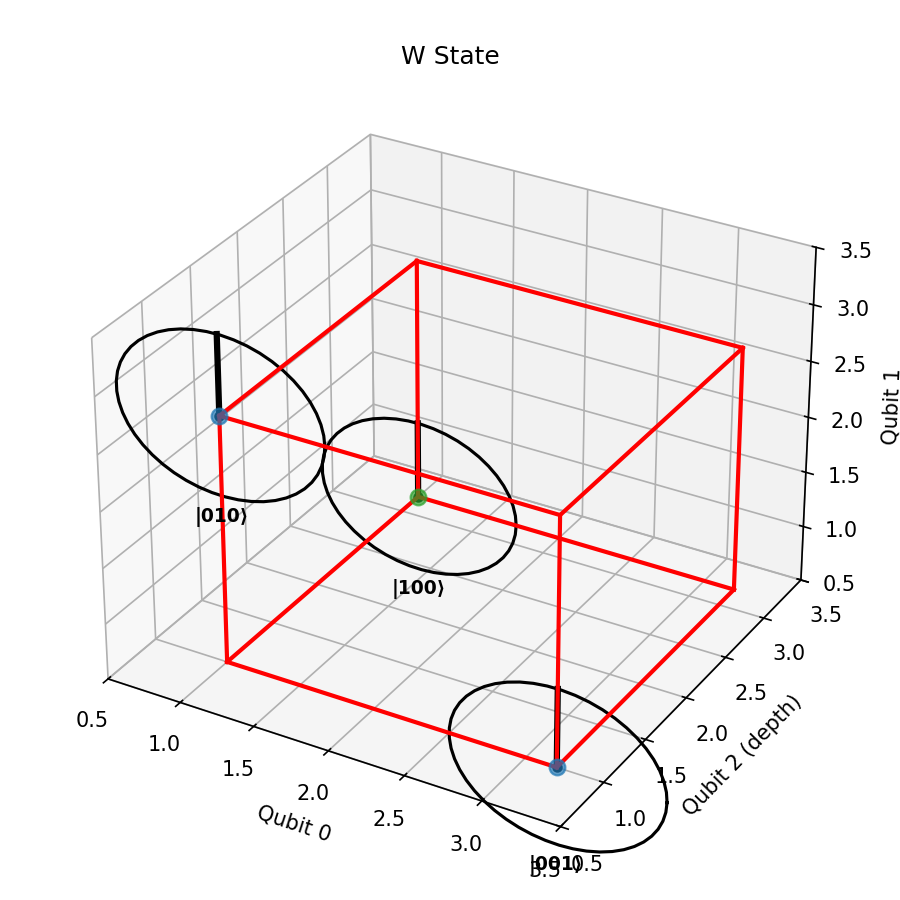
\includegraphics[width=0.6\linewidth]{figures_main/dcn-3qubit-w.png}
	\caption{Three-qubit W state $(|001\rangle + |010\rangle + |100\rangle)/\sqrt{3}$ in Dimensional Circular Notation. This state represents a different SLOCC entanglement class than GHZ. If any one qubit is measured, the remaining two qubits remain entangled. The DCN cube shows non-zero amplitudes on three corners sharing no common face.}
	\label{fig:dcn-3qubit-w}
\end{figure}
